Hansard is the official published report of oral and written UK Parliamentary proceedings. It is an edited verbatim report of speeeches in both the House of Commons and the House of Lords. Members' words are recorded by Hansard reporters and then edited to remove repetitions and obvious mistakes without changing the meaning. Reports of the latest proceedings are published online
% and updated during the day 
and can be read online back to 1988%
\footnote{For more information on Hansard and its history see \url{http://parldisc.jiscinvolve.org/wp/} and \url{http://www.parliament.uk/about/how/publications/hansard/}}.

These records are of importance for scholars of the development of the English language, of British politics and history, and are also used by community-focused organisations.  Historic records back to 1803 have been digitized in XML format and are publically available on the Historic Hansard web site created by the Commons and Lords Libraries and Millbank Systems. There one can search by word or phrase then filter results by speaker or House (Lords or Commons). 
% This is freely available online under an Office of Public Sector Information licence. 
% Together these web sites provide academic and non-academic communities with a significant amount of high-quality data. 
The Hansard corpus is one of the biggest humanities data sets in the UK but was limited in its use by being tagged only by speaker and date. To provide greater utility we wanted the speeches to be searchable by parts of speech (POS) and by topic. This would enhance this significant public material and expose it to new audiences
% within Higher Education, 
including linguists, discourse analysts, historians, digital humanists, and cultural scholars. 

We downloaded the XML corpus from the Historic Hansard site and standardised the XML coding in order to prepare it for the NLP toolchain. As well as POS tagging, we applied the USAS semantic tagger. Once these annotation steps were complete, we needed to produce word, POS and semantic frequency lists for each speech as per the standard Wmatrix tag wizard pipeline. Finally, in order to expose the key topics of each speech we compared each semantic frequency list to a standard reference corpus, the British National Corpus spoken sampler (one million words) using the log-likelihood statistic to find a set of key semantic tags.

% Glasgow downloaded the XML corpus from the Historic Hansard site, ran routines to standardise the XML coding and then passed the data to Lancaster. UCREL had the knowledge and experience to take on the complex tagging of this very large data set using their established software, the CLAWS part of speech tagger and the USAS semantic tagger.



% \begin{itemize}
%     \item Size
%         \begin{itemize}
%             \item 7545103 XML files in 48,482 directories comprising 2,271,985,142 words and 32.7952GiB of data [inc markup].
%             \item Word sizes: 40, 83, 147, 308, 1400 at 5\%, 25\%, 50\%, 75\% and 95\%.
            % > quantile(words$words, c(.05, .25, .50, .75, .95))
            %   5%  25%  50%  75%  95% 
            %   40   83  147  308 1400
%             \item Average filesize is 2.4KB
%             \item Totals and breakdowns
%         \end{itemize}
%     \item Format
%         \begin{itemize}
%             \item Individual files
%             \item folder structure and organisation (pertinent to later organisation/batching)
%         \end{itemize}
% \end{itemize}

% \subsection{Format}

The full 200-year collection is 2,271,985,142 words and 32.7%952
GiB of data, including mark-up. The corpus is split into 7,545,103 XML files, each representing one speech.
% a speech made in either house of the UK Parliament.  
These files are organised into a hierarchical directory structure by house and date, comprising 48,482 folders in total.  A sample of this structure is shown in Figure~\ref{fig:structure}.

\begin{figure}[h]
    \centering
    {
        \small
        \begin{Verbatim}[frame=single]
            Hansard
            +-- Commons
            |   +-- commons 1803-1820
            |   |   \-- commons
            |   |       +-- 1803
            |   |       |   +-- dec
            |   |       |   |   +-- 01
            |   |       |   |   +-- 02
            |   |       |   |   +-- 03
            |   |       |   |   +-- 05
            |   |       |   |   +-- ...
        \end{Verbatim} 
    }
    \caption{Sample directory layout}
    \label{fig:structure}
\end{figure}


\begin{figure}[h]
    \centering
    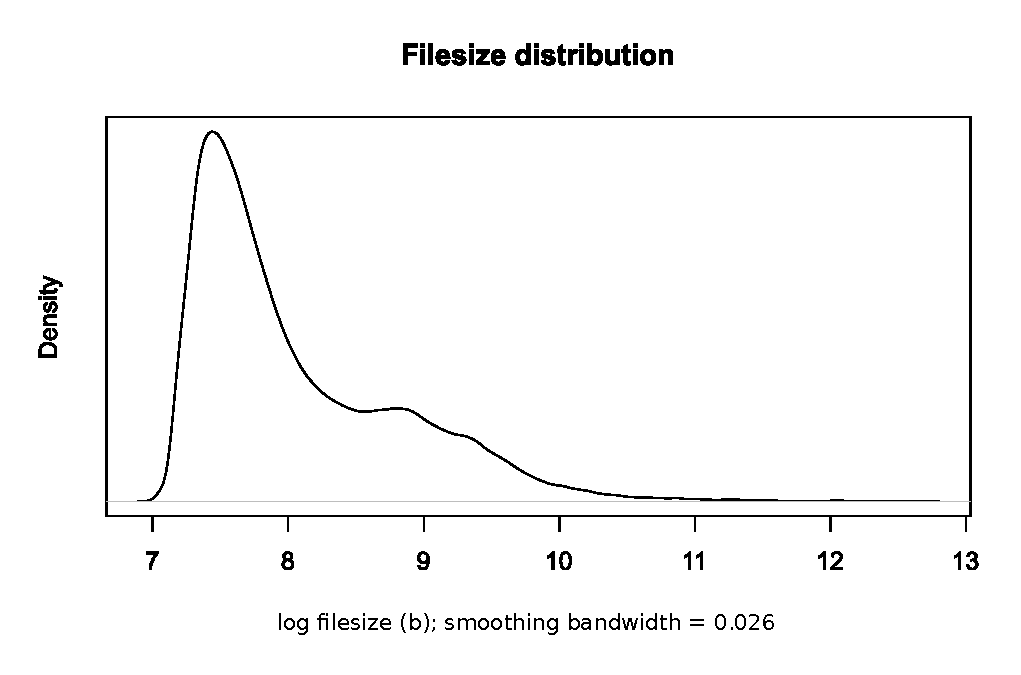
\includegraphics[width=0.5\textwidth]{filesize.eps}


    \begin{tabular}{ | r | c | c | c | c | c | }
        \hline
        Percentile & 5 & 25 & 50 & 75 & 95 \\ \hline
        Words & 40 & 83 & 147 & 308 & 1400 \\ \hline
    \end{tabular}

    \caption{Distribution of log filesizes for all corpus data, and word counts (without markup) for each file.}
    \label{fig:filesizes}
\end{figure}


% \dr{The XML format used contains annotations for X, Y and Z, and follows various conventions...  }

% The XML files themselves follow x format\todo{unsure of this, SW}. 

Figure~\ref{fig:filesizes} shows that filesizes are generally small, exhibiting a largely Zipfian distribution beyond the modal size of 1.8KB.\@ The median size is just 2.4KB, and the 95th percentile is 1.4MB.


% \begin{verbatim}
% > quantile(sizes$filesize, c(.05, .25, .50, .75, .95))
%    5%   25%   50%   75%   95% 
%  1411  1781  2443  5031 14013
% \end{verbatim}


% \subsection{Tagging}
% \begin{itemize}
%     \item What needed tagging
%     \item Which frequencies had to be built (per file/day/totals)
%     \item What work this contributed to
% \end{itemize}
